\documentclass[psamsfonts]{amsart}

%-------Packages---------
\usepackage{amssymb,amsfonts}
\usepackage{fullpage}
\usepackage{tikz-cd}
\usepackage{todonotes}
\usepackage{physics}
\usepackage[all,arc]{xy}
\usepackage{enumerate}
\usepackage{enumitem}
\usepackage{mathrsfs}
\usepackage{theoremref}
\usepackage{graphicx}
\usepackage[bookmarks]{hyperref}

%--------Theorem Environments--------
%theoremstyle{plain} --- default
\newtheorem{thm}{Theorem}[section]
\newtheorem{cor}[thm]{Corollary}
\newtheorem{prop}[thm]{Proposition}
\newtheorem{lem}[thm]{Lemma}
\newtheorem{conj}[thm]{Conjecture}
\newtheorem{quest}[thm]{Question}

\theoremstyle{definition}
\newtheorem{defn}[thm]{Definition}
\newtheorem{defns}[thm]{Definitions}
\newtheorem{con}[thm]{Construction}
\newtheorem{exmp}[thm]{Example}
\newtheorem{exmps}[thm]{Examples}
\newtheorem{notn}[thm]{Notation}
\newtheorem{notns}[thm]{Notations}
\newtheorem{addm}[thm]{Addendum}
\newtheorem*{exer}{Exercise}

\theoremstyle{remark}
\newtheorem{rem}[thm]{Remark}
\newtheorem{rems}[thm]{Remarks}
\newtheorem{warn}[thm]{Warning}
\newtheorem{sch}[thm]{Scholium}

\DeclareMathOperator{\Hom}{Hom}
\DeclareMathOperator{\Id}{Id}
\DeclareMathOperator{\End}{End}
\DeclareMathOperator{\ord}{ord}
\DeclareMathOperator{\Aut}{Aut}
\DeclareMathOperator{\Int}{int}
\DeclareMathOperator{\CP}{\mathbb{C}\mathbf{P}}

\makeatletter
\let\c@equation\c@thm
\makeatother
\numberwithin{equation}{section}

\bibliographystyle{plain}

\begin{document}

\title{Math 611 (Due 11/20)}
\author{Hidenori Shinohara}
\maketitle


\begin{exer}{(Problem 1)}
  \begin{itemize}
    \item
       \begin{figure}
       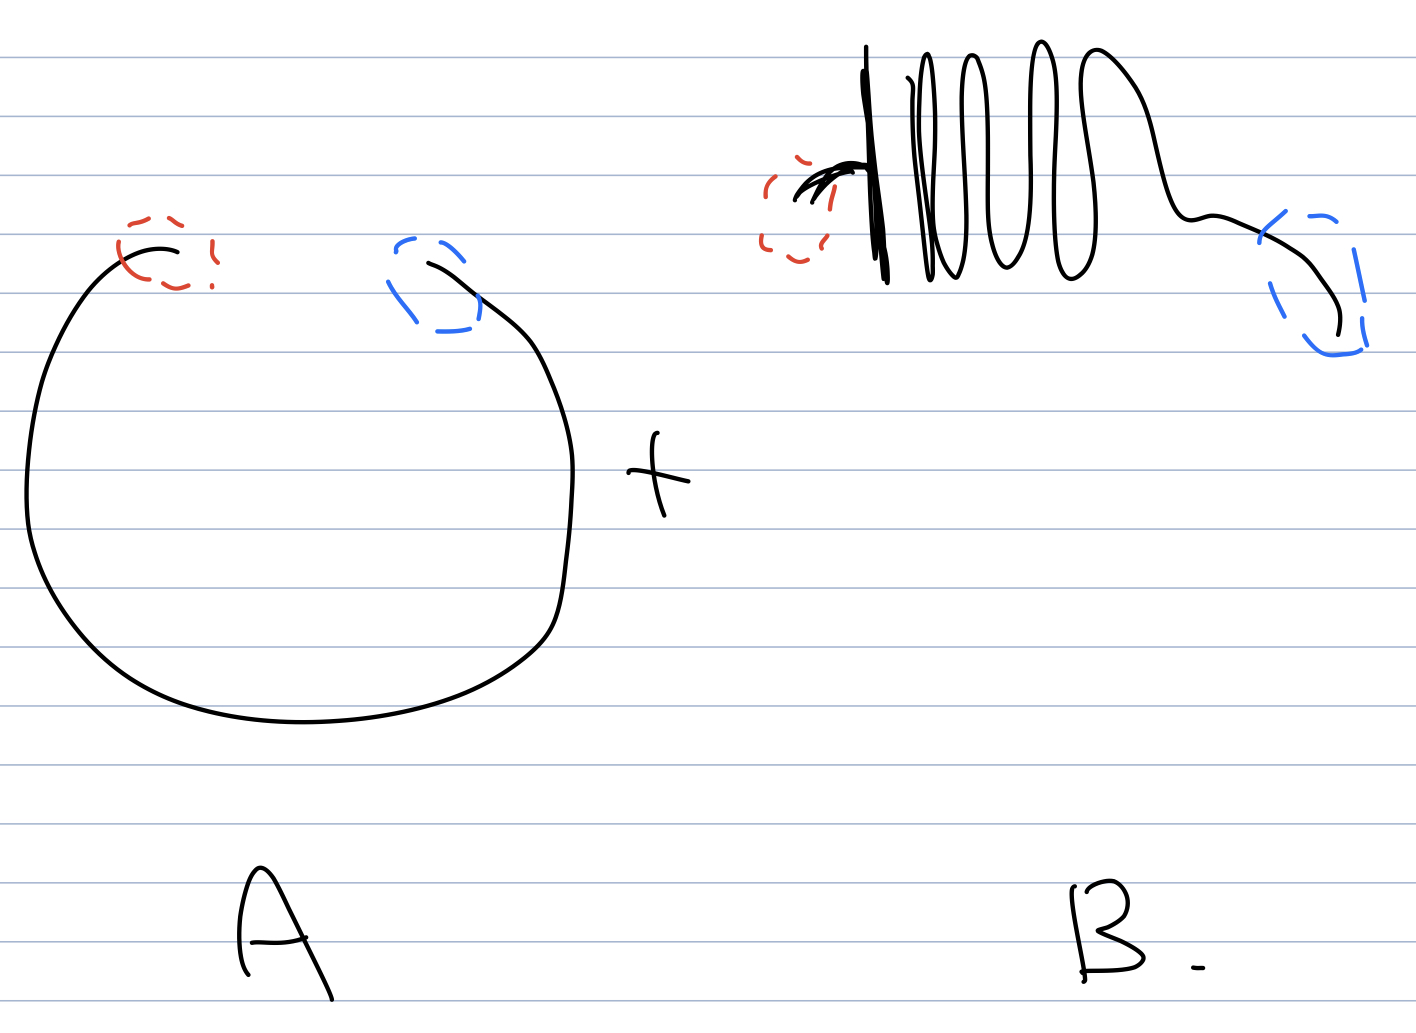
\includegraphics[width=.5\linewidth]{quasi.jpeg}
       \caption{Quasi circle}
       \label{fig:quasi}
       \end{figure}
       As shown in Figure \ref{fig:quasi}, we will let $A, B$ denote subspaces of $X$ such that $X = A \cup B$ and $A \cap B$ consists of two line segments.
       (Circled in the figure)
       Moreover, $X = \Int A \cup \Int B$.

       $H_n(A) = 0$ for all $n \geq 1$.
       By Proposition 2.6 (Hatcher), it suffices to consider each path component of $A \cap B$ separately.
       Each of them is homeomorphic to $\Delta^1$.
       Thus $H_n(A \cap B) = H_n(\Delta^1) \oplus H_n(\Delta^1) = 0$ for all $n \geq 1$.
       Using a similar argument, $H_n(B) = H_n(\Delta^1) \oplus H_n(\Delta^1) = 0$ for all $n \geq 1$.

       By the exact sequence $H_n(A) \oplus H_n(B) \rightarrow H_n(A \cup B) \rightarrow H_{n - 1}(A \cap B)$, $H_n(A \cup B) = 0$ for all $n \geq 2$.

       We will consider the exact sequence $0 \rightarrow H_1(A \cup B) \xrightarrow{\alpha} H_0(A \cap B) \xrightarrow{\beta} H_0(A) \oplus H_0(B)$.
       We have 0 because $H_1(A) \oplus H_1(B) = 0$.
       $H_0(A \cap B) = \mathbb{Z}^2, H_0(A) = \mathbb{Z}, H_0(B) = \mathbb{Z}^2$ by examining the number of path components.
       Let $a, b$ be generators of $H_0(A \cap B)$.
       Then $\beta(a, b) = (a + b, (a, b))$ because $a, b$ simply correspond to each path component in $A \cap B$.
       Therefore, $\beta$ is injective.
       Since $\alpha$ is injective by the exactness, $H_1(A \cup B) = \Im(\alpha) = \ker(\beta) = 0$.
       Hence, $H_1(X) = 0$.

       By examining the number of path components, $H_0(X) = \mathbb{Z}$.
     \item
       \begin{figure}
       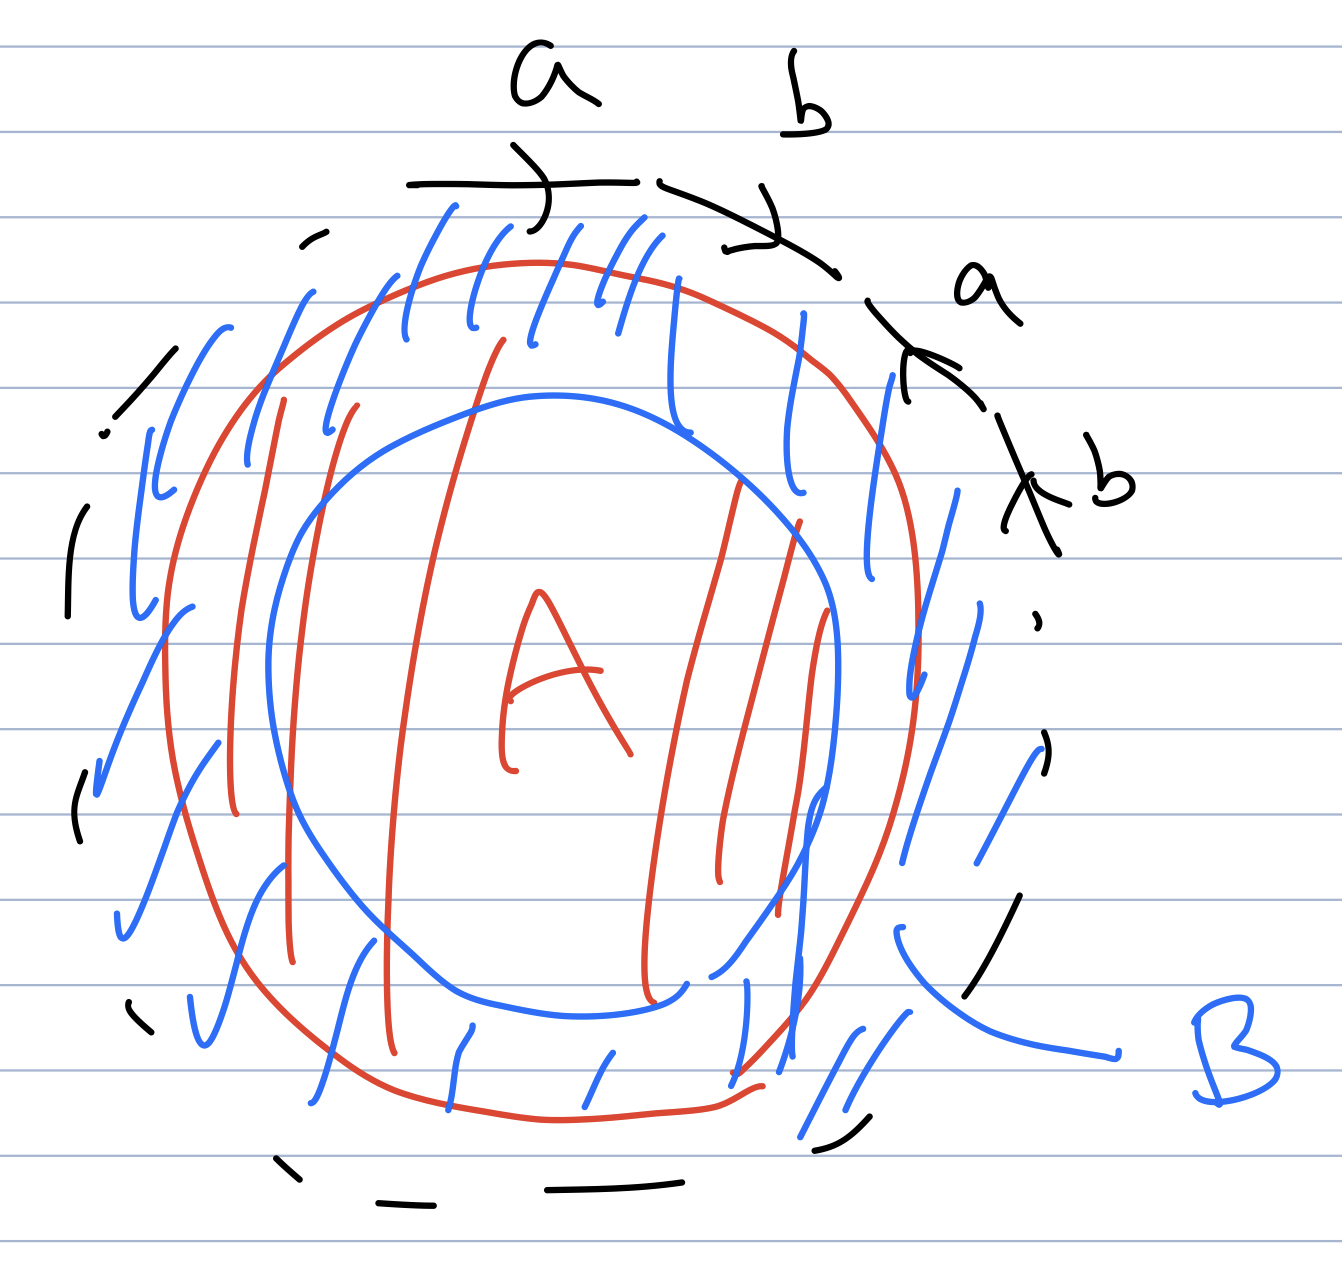
\includegraphics[width=.5\linewidth]{gtorus.jpeg}
       \caption{Genus $g$ surface}
       \label{fig:gtorus}
       \end{figure}
       Let $A, B$ denote the subspaces of $X$ as in Figure \ref{fig:gtorus}.
       Then $A \cap B$ is homotopy equivalent to $S^1$, and $B$ is homotopy equivalent to the wedge sum of $2g$ $S^1$'s.

       For any $n \geq 3$, $H_n(A) \oplus H_n(B) \rightarrow H_n(A \cup B) \rightarrow H_{n - 1}(A \cap B)$ shows that $H_n(A \cup B) = 0$ because $H_n(A) = H_n(B) = 0$ and $H_{n - 1}(A \cap B) = H_{n - 1}(S^1) = 0$.

       We have $0 \rightarrow \tilde{H}_2(A \cup B) \xrightarrow{\alpha} \tilde{H}_1(A \cap B) \xrightarrow{\beta} \tilde{H}_1(A) \oplus \tilde{H}_1(B) \xrightarrow{\gamma} \tilde{H}_1(A \cup B) \rightarrow 0$.
       We have 0's at the end because $\tilde{H}_2(A) \oplus \tilde{H}_2(B) = \tilde{H}_0(A \cap B) = 0$.
       We have $\tilde{H}_1(A \cap B) = \mathbb{Z}$ and $\tilde{H}_1(A) \oplus \tilde{H}_1(B) = \vee_{i=1}^{2g}\tilde{H}_1(S^1) = \mathbb{Z}^{2g}$.
       $\beta$ maps a generator $x$ into $(0, 0)$ because going around $A \cap B$ once cancels out all the generators of $\tilde{H}_1(B)$.
       For instance, in Figure \ref{fig:gtorus}, $\beta(x) = a + b - a - b + \cdots = 0$.
       Therefore, $\beta$ is the zero map.

       This implies that $\gamma$ is injective.
       By the exactness, $\gamma$ is surjective.
       Therefore, $\gamma$ is isomorphic, and thus $H_1(A \cup B) = \tilde{H}_1(A \cup B) = \mathbb{Z}^{2g}$.

       $\alpha$ is injective by the exactness, so $H_2(A \cup B) = \tilde{H}_2(A \cup B) = \Im(\alpha) = \tilde{H}_1(A \cap B) = \mathbb{Z}$.
       $H_0(A \cap B) = H_0(S^1) = \mathbb{Z}$.
     \item
       \begin{figure}
       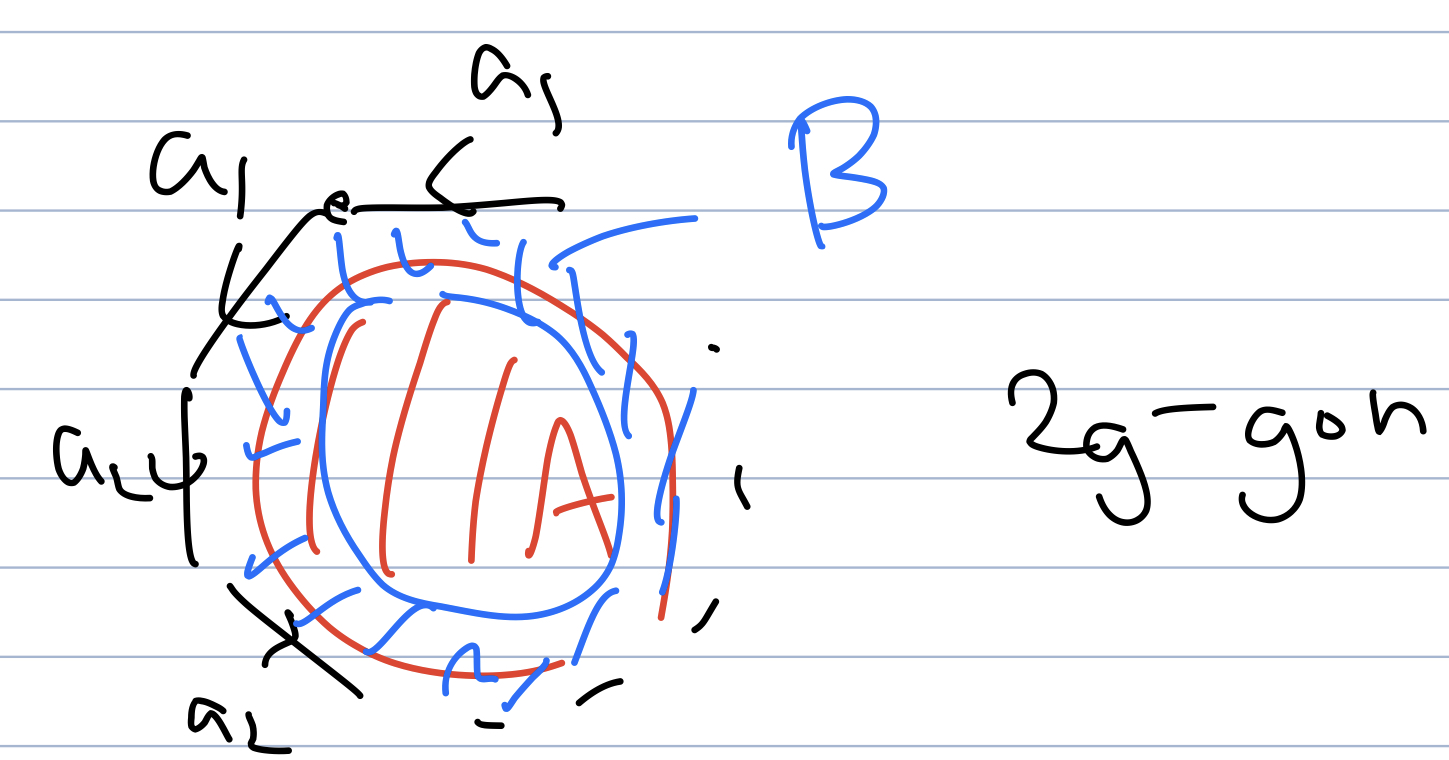
\includegraphics[width=.5\linewidth]{2g.jpeg}
       \caption{$N_g$}
       \label{fig:ng}
       \end{figure}
       Let $A, B$ denote the subspaces as in Figure \ref{fig:ng}.
       Then $A$ deformation retracts onto a point, $B$ is homotopy equivalent to $\vee_g \mathbb{R}P^1$, which is homotopy equivalent to $\vee_gS^1$.
       Finally, $A \cap B$ is homotopy equivalent to $S^1$.
       For any $n \geq 3$, $H_n(A) \oplus H_n(B) \rightarrow H_n(X) \rightarrow H_{n - 1}(A \cap B)$ is exact, and $H_n(A) = H_n(B) = H_{n - 1}(A \cap B) = 0$, so $H_n(X) = 0$.
       Consider $0 \rightarrow \tilde{H}_2(X) \xrightarrow{\alpha} \tilde{H}_1(A \cap B) \xrightarrow{\beta} \tilde{H}_1(A) \oplus \tilde{H}_1(B) \xrightarrow{\gamma} \tilde{H}_1(X) \rightarrow 0$.
       We have 0 at the end because $\tilde{H}_2(A) \oplus \tilde{H}_2(B) = \tilde{H}_0(A \cap B) = 0$.
       By exactness, $\alpha$ is injective and $\gamma$ is surjective.
       Let $a$ be a generator of $\tilde{H}_1(A \cap B) = \mathbb{Z}$.
       Then $\beta(a) = (0, 2(a_1 + \cdots + a_g))$ where $a_i$'s are generators of $\tilde{H}_1(B) = \mathbb{Z}^g$.
       \begin{itemize}
         \item
           Since $\beta$ is injective, so $0 = \ker(\beta) = \Im(\alpha) = \tilde{H}_2(X) = H_2(X)$.
         \item
           Since $\gamma$ is surjective, $\tilde{H}_1(X) = \tilde{H}_1(A) \oplus \tilde{H}_1(B) / \ker(\gamma)$.
           Since $\ker(\gamma) = \Im(\beta)$, this is $\ev{a_1, \cdots, a_g \mid 2(\sum a_i)}$.
           \begin{align*}
             H_1(X)
               &= \ev{a_1, \cdots, a_g \mid 2(a_1 + \cdots + a_g)} \\
               &= \ev{a_1 + \cdots + a_g, a_2, \cdots, a_g \mid 2(a_1 + \cdots + a_g)} \\
               &= \ev{b, a_2, \cdots, a_g \mid 2b} \\
               &= \mathbb{Z}^{g - 1} \oplus (\mathbb{Z}/2\mathbb{Z}).
           \end{align*}
         \item
           Since $X$ consists of one path component, $H_0(X) = \mathbb{Z}$.
       \end{itemize}
     \item
       \todo[inline,caption={}]{
         $\mathbb{R}P^3$.
       }
     \item
       Let $A = \CP^n - (0: \cdots : 0:1), B = \{ (a_1: \cdots : a_n:1) \mid a_i \in \mathbb{C} \}$.
       Since $\{ (0: \cdots :0:1) \}$ is closed, $A$ is an open set.
       Moreover, $(0: \cdots :0:1)$ is an interior point of $B$.
       Therefore, $\Int(A) \cup \Int(B) = \CP^n$.

       %$A = \{ (a_1: \cdots :a_n:0) \mid \{ a_1, \cdots, a_n \} \ne \{ 0 \} \} \coprod \{ (a_1: \cdots : a_n:1) \mid \{ a_1, \cdots, a_n \} \ne \{ 0 \} \}$.
       $A$ deformation retracts onto $\CP^{n - 1}$ by $F((a_1:\cdots :a_n:a_{n + 1}), t) = (a_1:\cdots : a_n:(1 - t)a_{n + 1})$.
       $B$ is homeomorphic to $\mathbb{C}^n$, which is contractible.
       Finally, $A \cap B = B \setminus (0 : \cdots : 0 : 1)$, which is homotopy equivalent to $\mathbb{C}^{n} - 0$.
       This is homotopy equivalent to $\mathbb{R}^{2n} - 0$, so it is $S^{2n - 1}$.

       We claim that $H_{2k}(\CP^n) = 0$ if $k > n$ and $\mathbb{Z}$ if $k \leq n$.
       We will use this to calculate $H_k(\CP^n)$ by induction on $n$.
       When $n = 0$, this is obvious because $\CP^0$ is a point.
       Suppose that we have shown this for some $n - 1$ where $n \in \mathbb{N}$.
       We will prove the case for $n$.
       \begin{itemize}
         \item
           We have the exact sequence $H_{2n}(A) \oplus H_{2n}(B) \rightarrow H_{2n}(X) \rightarrow H_{2n - 1}(A \cap B) \rightarrow H_{2n - 1}(A) \oplus H_{2n - 1}(B)$.
           $H_{2n}(A) = H_{2n - 1}(A) = 0$ by the inductive hypothesis since $A$ deformation retracts onto $\CP^{n - 1}$.
           $H_{2n}(B) = H_{2n - 1}(B) = 0$ because $B$ is contractible.
           By the exactness, $H_{2n}(X) \cong H_{2n - 1}(A \cap B) = \mathbb{Z}$ because $A \cap B$ is homotopy equivalent to $S^{2n - 1}$.
         \item
           We have the exact sequence $\tilde{H}_{2n - 1}(A) \oplus \tilde{H}_{2n - 1}(B) \rightarrow \tilde{H}_{2n - 1}(X) \rightarrow \tilde{H}_{2n - 2}(A \cap B)$.
           $\tilde{H}_{2n - 1}(A) = 0$ by the inductive hypothesis.
           $\tilde{H}_{2n - 1}(B) = 0$, and $\tilde{H}_{2n - 2}(A \cap B) = 0$, so $H_{2n - 1}(X) = \tilde{H}_{2n - 1}(X) = 0$.
       \end{itemize}

  \end{itemize}
\end{exer}

\begin{exer}{(Problem 28 (a))}
  Let $A, B$ be the Mobius strip and a torus with a small neighborhood around them so the strip and torus are contained in $A$ and $B$.
  For any $n \geq 3$, the exact sequence $H_n(A \cap B) \rightarrow H_n(A) \oplus H_n(B) \rightarrow H_n(X) \rightarrow H_{n - 1}(A \cap B)$ implies that $H_n(X) \cong H_n(A) \oplus H_n(B) = 0 \oplus 0 = 0$ because the intersection $A \cap B$ is homotopic to $S^1$, so $H_n(A \cap B) = H_{n - 1}(A \cap B) = 0$.
  $H_0(X) = \mathbb{Z}$ because $X$ has only one path component.

  We will examine the LES

  \begin{align*}
    \tilde{H}_2(A \cap B) \rightarrow \tilde{H}_2(A) \oplus \tilde{H}_2(B) \xrightarrow{f_1} \tilde{H}_2(X) 
    \xrightarrow{f_2} \tilde{H}_1(A \cap B) \xrightarrow{f_3} \tilde{H}_1(A) \oplus \tilde{H}_1(B) \xrightarrow{f_4} \tilde{H}_1(X) 
    \rightarrow \tilde{H}_0(A \cap B).
  \end{align*}

  \begin{itemize}
    \item
      Sine $\tilde{H}_2(A \cap B) = 0$, so $f_1$ is injective.
    \item
      $\tilde{H}_1(A \cap B) = \mathbb{Z}$, and $f_3(1) = (2, (1, 0))$ because the intersection goes around the mobius strip twice while it only goes around the torus once.
      Then $f_3$ is injective, so $\Im(f_2) = \ker(f_3) = 0$.
      This implies that $\Im(f_1) = \ker(f_2) = H_2$, so $f_1$ is surjective.
  \end{itemize}

  Therefore, $f_1$ is bijective, so $H_2(X) = \tilde{H}_2(X) = \tilde{H}_2(A) \oplus \tilde{H}_2(B) = 0 \oplus \mathbb{Z} = \mathbb{Z}$.

  Finally, $f_4$'s surjectivity implies that 
  \begin{align*}
    \tilde{H}_1(X)
      &\cong \tilde{H}_1(A) \oplus \tilde{H}_1(B) / \ker(f_4) \\
      &= \mathbb{Z} \oplus \mathbb{Z}^2 / \ev{(2, (1, 0))} \\
      &\cong \ev{a, b, c} / \ev{2a + b} \\
      &\cong \ev{a, b, c \mid 2a + b} \\
      &\cong \ev{a, -2a, c} \\
      &\cong \ev{a, c} = \mathbb{Z} \oplus \mathbb{Z}.
  \end{align*}
  Thus $H_1(X) = \mathbb{Z} \oplus \mathbb{Z}$.
\end{exer}

\begin{exer}{(Problem 28 (b))}
  Let $A, B$ be the Mobius strip and $\mathbb{R}P^2$ with a small neighborhood around them so the strip and $\mathbb{R}P^2$ are contained in $A$ and $B$.
  For any $n \geq 3$, the exact sequence $H_n(A \cap B) \rightarrow H_n(A) \oplus H_n(B) \rightarrow H_n(X) \rightarrow H_{n - 1}(A \cap B)$ implies that $H_n(X) \cong H_n(A) \oplus H_n(B) = 0 \oplus 0 = 0$ because the intersection $A \cap B$ is homotopic to $S^1$, so $H_n(A \cap B) = H_{n - 1}(A \cap B) = 0$.
  Since $X = A \cup B$ has one path component, $H_0(X) = \mathbb{Z}$.
  We will consider the LES

  \begin{align*}
    \tilde{H}_2(A) \oplus \tilde{H}_2(B) \xrightarrow{f_1} \tilde{H}_2(X) 
    \xrightarrow{f_2} \tilde{H}_1(A \cap B) \xrightarrow{f_3} \tilde{H}_1(A) \oplus \tilde{H}_1(B) \xrightarrow{f_4} \tilde{H}_1(X) 
    \rightarrow \tilde{H}_0(A \cap B).
  \end{align*}

  $\tilde{H}_1(A \cap B) = \mathbb{Z}$, and $f_3$ maps $1$ to $(2, 1)$ because the generator wraps around the Mobius strip twice and the $\mathbb{R}P^2$ once.
  Then $f_3$ is injective, so $f_2$ is the zero map.
  In other words, $\ker(f_2) = \tilde{H}_2(X)$, so $f_1$ is surjective.
  Since $\tilde{H}_2(A) \oplus \tilde{H}_2(B) = 0$, $\tilde{H}_2(X) = 0$.
  Thus $H_2(X) = 0$.

  By the first isomorphism theorem and exactness,

  \begin{align*}
    \tilde{H}_1(X)
      &= \tilde{H}_1(A) \oplus \tilde{H}_1(B) / \ker(f_4) \\
      &= (\mathbb{Z} \oplus \mathbb{Z}/2\mathbb{Z}) / \ev{(2, 1)} \\
      &\cong \ev{a, b \mid 2b}  / \ev{2a + b} \\
      &= \ev{a, b \mid 2b, 2a + b} \\
      &= \ev{a, -2a \mid 2(-2a)} \\
      &= \ev{a \mid 4a} \\
      &= \mathbb{Z}_4.
  \end{align*}
  Therefore, $H_1(X) = \mathbb{Z}_4$.
\end{exer}

\begin{exer}{(Problem 29)}
  As shown earlier,
  \begin{align*}
    H_n(M_g) &= \begin{cases}
      \mathbb{Z}^{2g} & (n = 1) \\
      \mathbb{Z} & (n = 0, 2) \\
      0 & (n \geq 3).
    \end{cases}
  \end{align*}
  Let $R_1, R_2$ be the first and second $R$ with a small neighborhood around them.
  Then $X = R_1 \cup R_2$ and $R_1 \cap R_2$ is homotopy equivalent to $M_g$.
  Let $n \geq 3$.
  Consider the sequence 
  \begin{align*}
    H_n(R_1) \oplus H_n(R_2) \rightarrow H_n(X) \rightarrow H_{n - 1}(R_1 \cap R_2) \rightarrow H_{n - 1}(R_1) \oplus H_{n - 1}(R_2).
  \end{align*}
  A solid $g$-torus deformation retracts to the wedge sum of $g$ $S^1$'s.
  $H_n(R_1) = H_n(R_2) = \oplus_{i=1}^g H_n(S^1) = 0$ for $n \geq 2$.
  By the exactness, we have $H_n(X) = H_{n - 1}(R_1 \cap R_2) = H_{n - 1}(M_g)$.
  Therefore, $H_n(X) = 0$ for $n \geq 4$, and $H_3(X) = \mathbb{Z}$.
  $H_0(X) = \mathbb{Z}$ because $X$ contains only one path component.

  Consider the sequence 
  \begin{align*}
    \tilde{H}_2(R_1) \oplus \tilde{H}_2(R_2) \rightarrow \tilde{H}_2(X) \xrightarrow{\alpha} \tilde{H}_{1}(R_1 \cap R_2) \xrightarrow{\beta} \tilde{H}_{1}(R_1) \oplus \tilde{H}_{1}(R_2) \xrightarrow{\gamma} \tilde{H}_1(X) \rightarrow \tilde{H}_0(R_1 \cap R_2).
  \end{align*}

  Then this is equivalent to

  \begin{align*}
    0 \rightarrow \tilde{H}_2(X) \xrightarrow{\alpha} \tilde{H}_{1}(R_1 \cap R_2) \xrightarrow{\beta} \tilde{H}_{1}(R_1) \oplus \tilde{H}_{1}(R_2) \xrightarrow{\gamma} \tilde{H}_1(X) \rightarrow 0.
  \end{align*}

  By the exactness, $\alpha$ is injective and $\gamma$ is surjective.
  Let $a_1, \cdots, a_g, b_1, \cdots, b_g$ be generators of $\tilde{H}_1(R_1 \cap R_2)$ where $a_i$ wraps around the $i$th ``arm"(or ``handle") and $b_i$ wraps around the $i$th ``hole".
  Then $\beta(a_i) = (0, 0)$ because in $R_1$ and $R_2$, each of which is a solid torus, the ``arm" gets filled in.
  On the other hand, $\beta(b_i) = (b_i, b_i)$ for each $i$.

  \begin{align*}
    H_1(X)
      &= \tilde{H}_1(X) \\
      &= \Im(\gamma) \\
      &= \tilde{H}_1(R_1) \oplus \tilde{H}_1(R_2) / \ker(\gamma) \\
      &= \tilde{H}_1(R_1) \oplus \tilde{H}_1(R_2) / \Im(\beta) \\
      &= \ev{b_1, \cdots, b_g, b_1', \cdots, b_g'} / \ev{b_1 + b_1', \cdots, b_g + b_g'} \\
      &= \ev{b_1, \cdots, b_g} \\
      &= \mathbb{Z}^g.
  \end{align*}

  Since $\alpha$ is injective, $\Im(\alpha)$ is isomorphic to $\tilde{H}_2(X)$.
  Thus $H_2(X) = \tilde{H}_2(X) = \Im(\alpha) = \ker(\beta) = \ev{a_1, \cdots, a_g} = \mathbb{Z}^g$.

  \begin{itemize}
    \item
      For $n \geq 4$, we have $H_n(R) \rightarrow H_n(R, M_g) \rightarrow H_{n - 1}(M_g)$.
      As shown earlier, $H_n(R) = H_{n - 1}(M_g) = 0$, so the exactness implies that $H_n(R, M_g) = 0$.
    \item
      We will consider $H_3(R) \rightarrow H_3(R, M_g) \rightarrow H_2(M_g) \rightarrow H_2(R)$.
      $H_3(R) = H_2(R) = 0$, so $H_3(R, M_g) = H_2(M_g)$ by the exactness.
      Thus $H_3(R, M_g) = \mathbb{Z}$.
    \item
      We will consider $0 \rightarrow \tilde{H}_2(R, M_g) \xrightarrow{\alpha} \tilde{H}_1(M_g) \xrightarrow{\beta} \tilde{H}_1(R) \xrightarrow{\gamma} \tilde{H}_1(R, M_g) \rightarrow 0$.
      (We have 0 on both ends because $\tilde{H}_2(R) = \tilde{H}_0(M_g) = 0$.
      Let $a_i, b_i$ be generators of $\tilde{H}_1{M_g}$ such that $a_i$'s wrap around the handles and $b_i$'s wrap around the holes.
      Using the same discussion as above, $a_i \mapsto 0$ and $b_i \mapsto b_i$ by $\beta$.
      \begin{itemize}
        \item
          By the exactness, $\alpha$ is injective.
          Thus $\tilde{H}_2(R, M_g) = \Im(\alpha) = \ker(\beta) = \ev{a_1, \cdots, a_g}$.
          Therefore, $\tilde{H}_2(R, M_g) = \mathbb{Z}^g$.
        \item
          By the exactness, $\gamma$ is surjective.
          $\tilde{H}_1(R, M_g) = \Im(\gamma) = \tilde{H}_1(R) / \ker(\gamma) = \tilde{H}_1(R) / \Im(\beta)$.
          $\tilde{H}_1(R)$ is generated by $b_1, \cdots, b_g$ as it deformation retracts to $S^1 \vee \cdots \vee S^1$, so $\beta$ is surjective.
          Therefore, $\tilde{H}_1(R, M_g) = 0$.
      \end{itemize}
    \item
      $0 = H_1(R, M_g) \rightarrow H_0(M_g) \xrightarrow{f} H_0(R) \rightarrow H_0(R, M_g)$ is exact.
      Moreover, $f$ must be an isomorphism because both $M_g$ and $R$ consist of one path component.
      Therefore, the exactness implies $H_0(R, M_g) = 0$.
  \end{itemize}
\end{exer}

\end{document}


